% Modified from https://www.overleaf.com/latex/templates/university-of-melbourne-poster-template/swfmhrpvfryh
% The original author is  Jiyu Chen
% modified by Qi Dang
% Last Modified: 2021-01-10

% Modified from https://www.overleaf.com/latex/templates/stockholm-university-poster-template/xsrhnggqmcsx
% The author, Qi Dang, based their work on that of Jiyu Chen, as mentioned above.
% Modified by Jason Balaci
% Last Modified: 2022-04-12

% Modified from https://github.com/JacquesCarette/Drasil/blob/master/People/Jason/poster/poster.tex
% The author, Jason Balaci, changed it to the McMaster version from Qi Dang, who based their work on that of Jiyu Chen, as mentioned above.
% Modified by Michael (Minsung) Kim
% Last Modified: 2024-03-25

\documentclass[18pt,margin=1in,innermargin=-1in,blockverticalspace=-0.1in]{tikzposter}
\geometry{paperwidth=48in,paperheight=36in}

\usepackage{xparse}

\usepackage[canadian]{babel}

\usepackage[utf8]{inputenc}
\usepackage[T1]{fontenc}

\usepackage{blindtext}

\usepackage{amsmath}
\usepackage{amsfonts}
\usepackage{amsthm}
\usepackage{amssymb}
\usepackage{mathrsfs}
\usepackage{graphicx}
\usepackage{adjustbox}
\usepackage{enumitem}
\usepackage{csquotes}
\usepackage[backend=biber,style=numeric]{biblatex}

\usepackage{tikz}
\usetikzlibrary{cd}
\usetikzlibrary{babel} % Make sure quiver/tikz uses babel

\usepackage{mwe} % for placeholder images

\usepackage{McMasterTheme}
\tikzposterlatexaffectionproofoff
\usetheme{McMasterTheme}
\usecolorstyle{McMasterStyle}
\usetitlestyle{Filled}

\usepackage[scaled]{helvet}
\renewcommand\familydefault{\sfdefault} 
\usepackage[T1]{fontenc}

\title{Capstone Project Team 2: CampusConnections}
\author{Abhiram Neelamraju, Firas Elayan, Matthew Miller, Michael Kim, Waseef Nayeem, Zihao Du}
\institute{Department of Computing and Software, McMaster University}
\titlegraphic{
\includegraphics[width=0.16\textwidth]{assets/mcm-cas_left-wht_eps.eps}}
\projectlogo{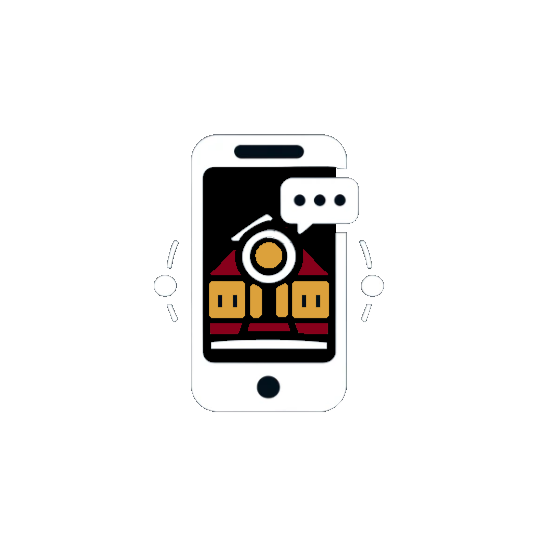
\includegraphics[width=0.06\textwidth]{assets/CampusConnections_logo.png}}

% begin document
\begin{document}

\maketitle

\centering
\begin{columns}
    %----------------------------------
    %- First Column
    %----------------------------------
    \column{0.1}

    \block{What is CampusConnections?}{CampusConnections is an Android based mobile application that provides students and visitors of McMaster University with location-based campus information, 
                                       engaging interactions with the campus through Augmented Reality (AR), and a sense of connectedness with the McMaster community. 
                                       The app is built using Unity, leveraging a mobile device’s camera and GPS sensor. With the main campus map view, 
                                       the app let users explore events and lectures happening on campus, as well as search for specific information, 
                                       which can be shared with friends easily through our built-in friend system. The AR functionality allows users to interact with the buildings on campus with their camera, 
                                       and view location-based information in real time. The main campus map view also visualizes all users’ location information (with user consent) on the map, 
                                       to raise awareness, foster a sense of community, and hence strengthen the social connections on campus.}

    \block{Software Architecture}{
    \begin{tabular}{c}
        \textbf{Component Diagram} \\
        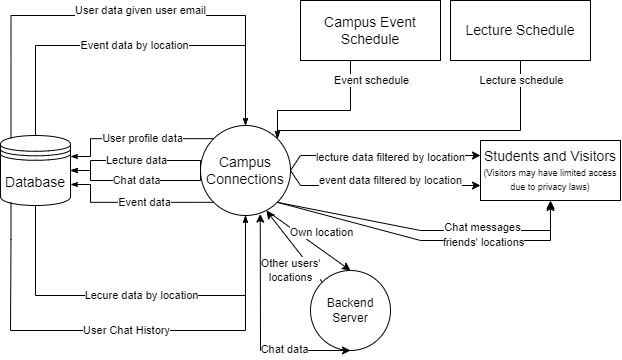
\includegraphics[width=0.4\textwidth]{assets/Context_Diagram.png}  \\
        \textbf{Tools Used} \\
        \begin{tabular}{cccc}
            
\includegraphics[width=0.1\textwidth]{assets/GitHub-logo.png}  &
            
\includegraphics[width=0.1\textwidth]{assets/firebase-logo.png} &
            
\includegraphics[width=0.1\textwidth]{assets/mapbox-logo.png} &
            
\includegraphics[width=0.1\textwidth]{assets/vuforia-logo.png}
        \end{tabular}
    \end{tabular}
}

    %----------------------------------
    %- Second Column
    %----------------------------------
    \column{0.1}%0.46
    \block{Key Features}{
        \vspace{-1em}
        \centering
        \begin{tabular}{ccc}
            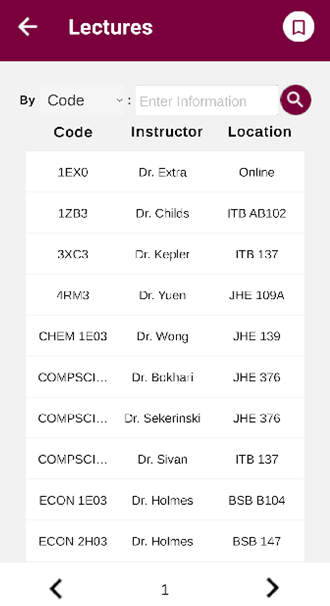
\includegraphics[width=0.1\textwidth,height=0.25\textheight]{assets/Lectures_screen.png} & 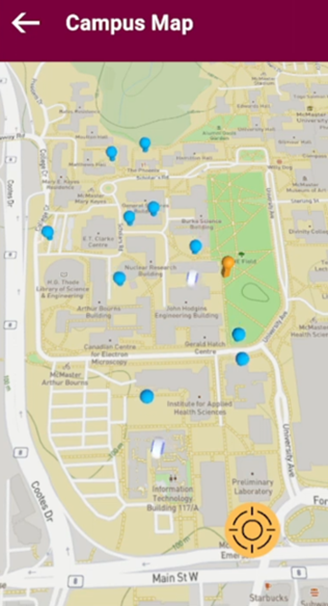
\includegraphics[width=0.1\textwidth,height=0.25\textheight]{assets/Map.png} & 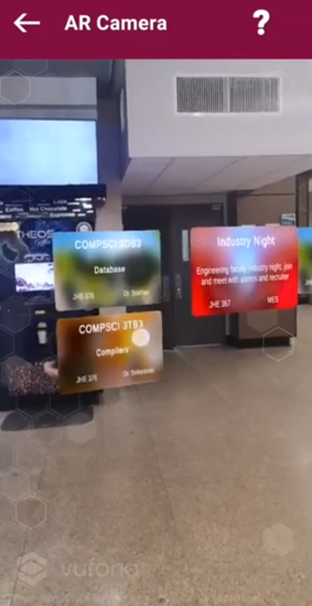
\includegraphics[width=0.1\textwidth,height=0.25\textheight]{assets/AR.png} \\
            Lecture Search & Location & AR \\
            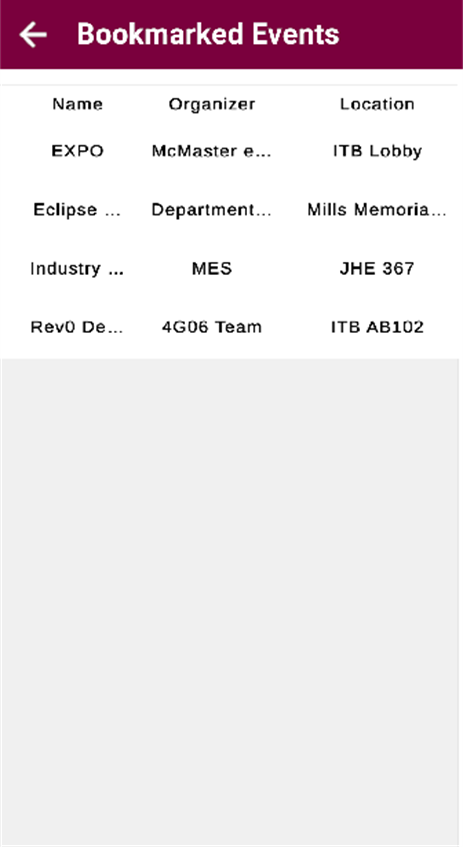
\includegraphics[width=0.1\textwidth,height=0.25\textheight]{assets/Bookmarked_events.png} & 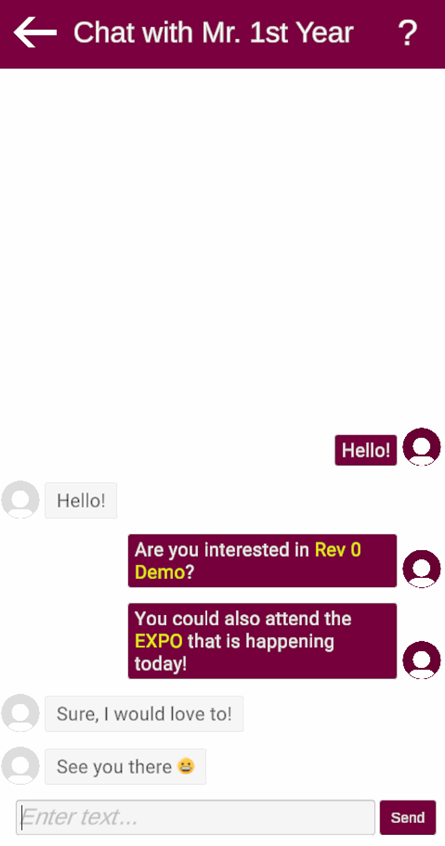
\includegraphics[width=0.1\textwidth,height=0.25\textheight]{assets/chat.png} & 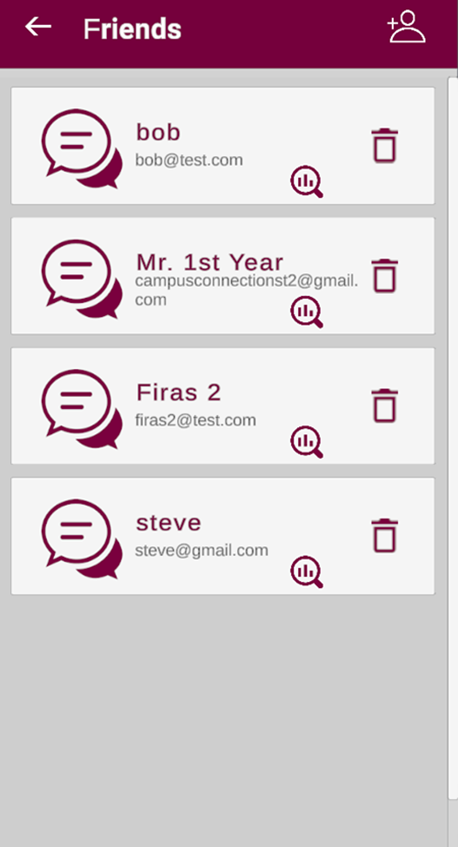
\includegraphics[width=0.1\textwidth,height=0.25\textheight]{assets/friends.png} \\
            Bookmarked Events & Chat & Friends
        \end{tabular}

    }

    %----------------------------------
    %- Third Column
    %----------------------------------
    \column{0.5}%0.5

    \block{Key Benefits}{
        \vspace{-0.8em}
        \textbf{Scalability}: New data and users can be easily added or changed. AR elements can be added by pushing a single unity package using Vuforia. \\
        \textbf{Centralization}: One location for admins and users to access all the information they need at McMaster. \\
        \textbf{Ease of Use}: Using simple designs with McMaster style makes it familiar to all user on campus. \\
        \textbf{Discoverability}: With AR, users can find events and friends with ease throughout the campus. \\
    }

    \block{Future Continuation}{
        \vspace{-0.8em}
        \begin{itemize}
            \item Heat map of user locations in campus to display which study spaces are occupied and which are available.
            \item Better user interaction by allowing other users to discover nearby users and interact with event attendees more easily.
            \item Generalization of the application to be used in other campuses or venues.
        \end{itemize}
    }

    \block{Acknowledgements}{
        \vspace{-1em}
        \begin{itemize}
            \item To Dr. Irene Yuan, supervisor of this project and for all her help in designing and improving the usability of the application.
            \item To Dr. Spencer Smith and Samuel Crawford for helping us through the project and keeping us on a working schedule.
        \end{itemize}
    }

    \block{Team Members}{
        \vspace{-0.5em}
        \centering
        \begin{tabular}{cccccc}
             &
             &
            \includegraphics[width=0.05\textwidth,height=0.08\textheight]{assets/Matthew.png} &
            \includegraphics[width=0.05\textwidth,height=0.08\textheight]{assets/Michael.png} &
            \includegraphics[width=0.05\textwidth,height=0.08\textheight]{assets/Waseef.png} &
            \includegraphics[width=0.05\textwidth,height=0.08\textheight]{assets/Zihao.png} \\
            \small Abhiram Neelamraju & \small Firas Elayan & \small Matthew Miller & \small Michael Kim & \small Waseef Nayeem & \small Zihao Du
        \end{tabular}
    }

\end{columns}

\end{document}
